\section*{Лекція 15: Застосування Python. Створення гри за допомогою Pygame}

\subsection{Знайомство з Pygame} 

\begin{frame}
\frametitle{Що таке Pygame?}
Pygame — набір модулів для Python, створений для розробки відеоігор. Включає в себе бібліотеки комп'ютерної графіки і звуку на базі мультимедійної бібліотеки SDL. 

\begin{figure}
  \begin{center}
    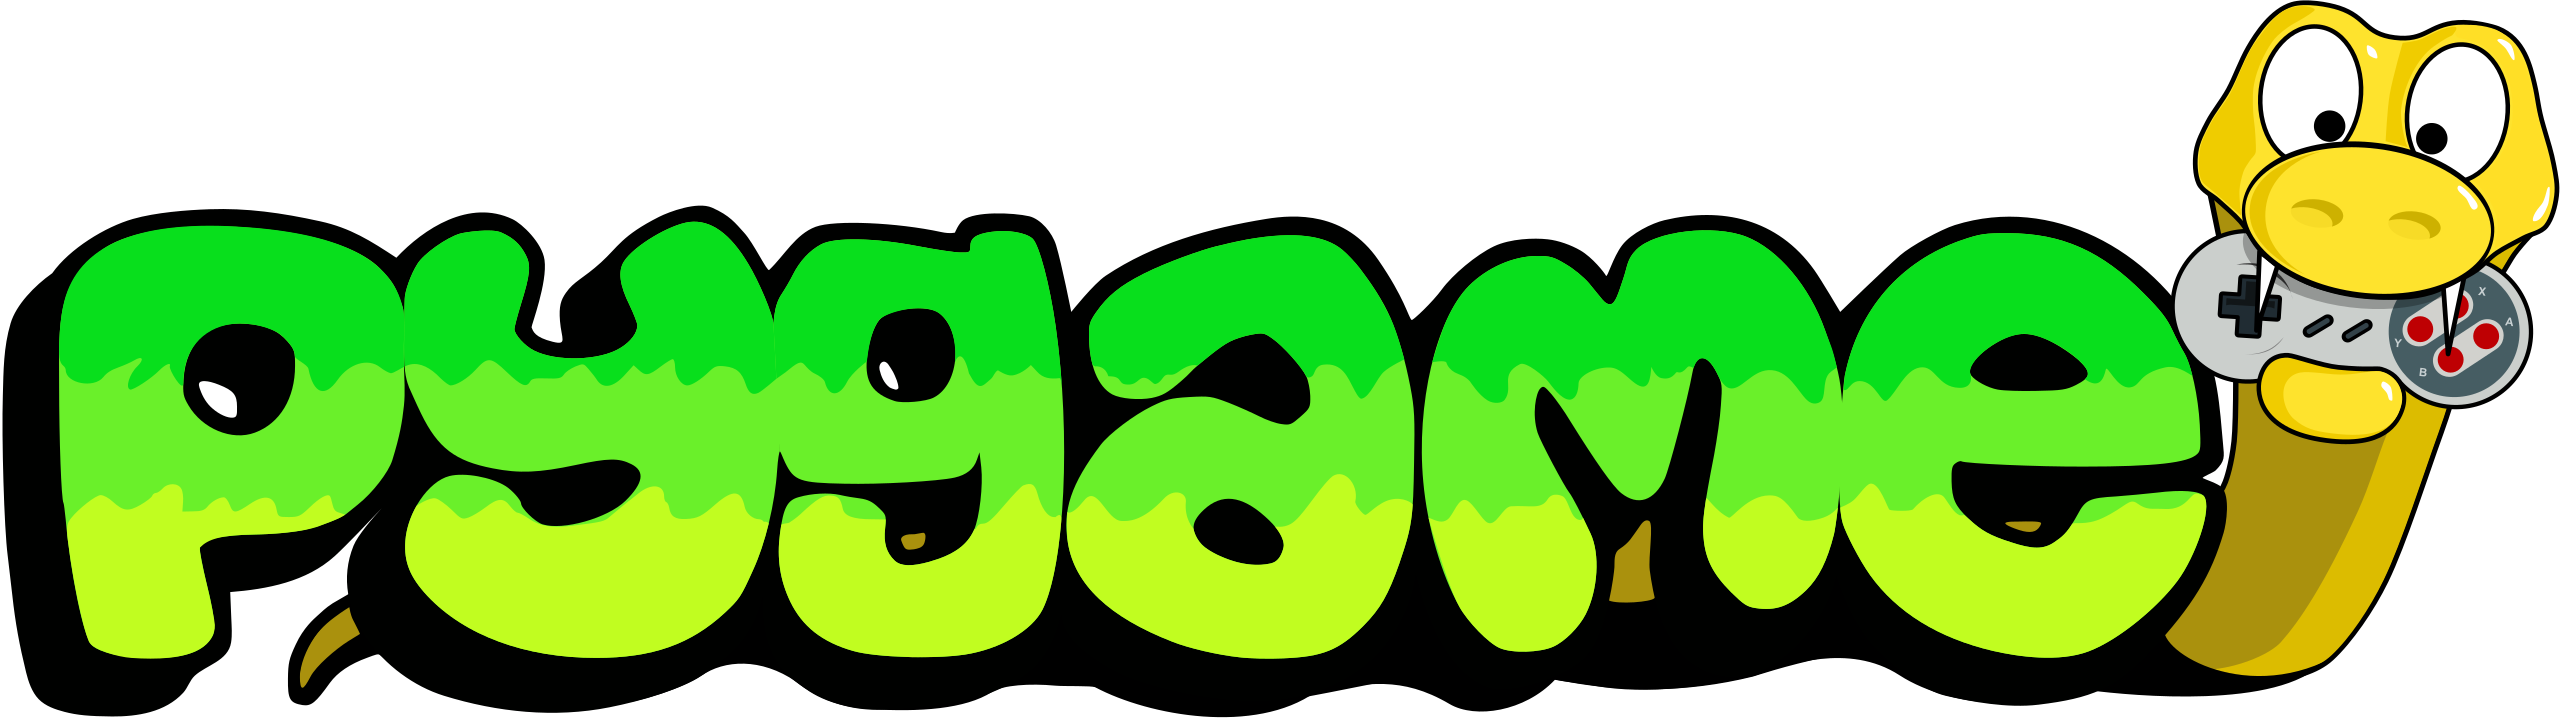
\includegraphics[width=0.75\textwidth,height=0.4\textheight]{pictures/pygame.png}
  \caption{\href{https://www.pygame.org/news}{Pygame}}
\label{function}
  \end{center}
\end{figure}

\end{frame}

\begin{frame}
\frametitle{Встановлення та тестування Pygame}
Для встановлення Pygame наберіть в командному рядку команду

\begin{center}
\texttt{pip install pygame }
\end{center}

\vspace{0.5cm}
Тестування Pygame:

\texttt{import pygame}

\texttt{pygame.init()}

\texttt{win = pygame.display.set\_mode((500, 500))}
\end{frame}

\subsection{Створення та переміщення гравця} 

\begin{frame}
\frametitle{Головний цикл}

Головний цикл перевіряє всі події в грі. 

\vspace{0.5cm}

\texttt{run = True}

\texttt{while run:}

\texttt{~~~~pygame.time.delay(100)}

\texttt{~~~~for event in pygame.event.get():}

\texttt{~~~~~~~~if event.type == pygame.QUIT:}

\texttt{~~~~~~~~~~~~run = False}

\texttt{pygame.quit()}
\end{frame}

\begin{frame}
\frametitle{Створення гравця}

Для створення гравця всередині основного циклу малюємо прямокутник. Для молелювання переміщення гравця малюванням прямокутника вікно заповнюється чорним кольором.

\texttt{win.fill((0, 0, 0))}

\texttt{pygame.draw.rect(win, (0, 0, 255), (x, y, width, height))}

\texttt{pygame.display.update()}
\end{frame}

\begin{frame}
\frametitle{Моделювання переміщення гравця}
Записуємо до словника keys натиснуті клавіші

\texttt{keys = pygame.key.get\_pressed()}

У випадку якщо натиснуто одну із клавіш із стрілочками (K\_LEFT, K\_RIGHT, K\_UP або K\_DOWN) збільшуємо або зменшуємо відповідну координату 

\texttt{if keys[pygame.K\_LEFT]:}

\texttt{~~~~x -= speed}
\end{frame}

\subsection{Додавання границь та стрибки}
\begin{frame}
\frametitle{Додавання границь}
Для додавання границь слід обмежувати переміщення гравця додатковими умовами. Координати (0, 0) відповідають верхньому лівому куту. Приклад для переміщення ліворуч 

\texttt{if keys[pygame.K\_LEFT] and x > bound:}

\texttt{~~~~x -= speed}

Приклад для переміщення праворуч

\texttt{if keys[pygame.K\_RIGHT] and x < WIDTH - width - bound:}

\texttt{~~~~x += speed}
\end{frame}

\begin{frame}
\frametitle{Підготовка до стрибка}
Введемо змінні \texttt{isJump = False} (\texttt{True} - гравець в цей момент стрибає) та \texttt{JumpCount = g} (параметр стрибка, \texttt{g = 10}). Переміщення по координаті \texttt{y} відбувається якщо гравець не стрибає, при натисненні пробілу здійснюється стрибок:  

\texttt{if not isJump:}

\texttt{~~~~Переміщення UP та DOWN.}  
      
\texttt{~~~~if keys[pygame.K\_SPACE]:}

\texttt{~~~~~~~~isJump = True}

\texttt{else:}

\texttt{~~~~pass}
        
\end{frame}

\begin{frame}
\frametitle{Реалізація стрибка}
Гравець стрибає за параболічним законом. 

\texttt{if JumpCount >= -g:}

\texttt{~~~~if JumpCount < 0:}

\texttt{~~~~~~~~y += (JumpCount ** 2) / 2}

\texttt{~~~~else:}

\texttt{~~~~~~~~y -= (JumpCount ** 2) / 2}

\texttt{~~~~JumpCount -= 1}

\texttt{else:}

\texttt{~~~~isJump = False}

\texttt{~~~~JumpCount = g}        
\end{frame}

\subsection{Анімація та спрайти}

\begin{frame}
\frametitle{Анімація}
Для анімації та пересування кадри спрацьовують n разів щосекунди. Частота оновлення  \texttt{c2s = 30} кадрів за секунду. Використаємо клас \texttt{pygame.time.Clock} та його метод \texttt{tick()}.

def drawWindow():

~~~~win.fill((0, 0, 0))

~~~~pygame.draw.rect(win, (0, 0, 255), (x, y, width, height))

~~~~pygame.display.update()

while run:

~~~~clock.tick(c2s)

~~~~...

~~~~drawWindow()

\end{frame}

\begin{frame}
\frametitle{Додавання зображень до гри}
Функція \texttt{load} дозволяє завантажувати картинки (спрайти) до гри. Завантажимо спрайти для імітації переміщення гравця праворуч та ліворуч:

\texttt{walkRight = [pygame.image.load('right\_1.png'), ... ]}

\texttt{walkLeft = [pygame.image.load('left\_1.png'), ... ]}
 
А також для нерухомого гравця та тлу:
 
\texttt{playerStand = pygame.image.load('idle.png')}

\texttt{bg = pygame.image.load('bg.jpg')} 
\end{frame}

\begin{frame}
\frametitle{Функція drawWindow. Додавання тла, оновлення щосекунди}
\texttt{def drawWindow():}

\texttt{~~~~global animCount}

\texttt{~~~~win.blit(bg, (0, 0))}

\texttt{~~~~if animCount + 1 >= c2s:} 

\texttt{~~~~~~~~animCount = 0}
    
~~~~\textit{Малювання гравця}
        
\texttt{~~~~pygame.display.update()}    
\end{frame}

\begin{frame}
\frametitle{Оновлення блоку переміщення гравця}
При переміщенні ліворуч чи праворуч оновлюємо змінні left та right, інакше - стоїмо.

\texttt{if keys[pygame.K\_LEFT] and x > bound:}

\texttt{~~~~x -= speed}

\texttt{~~~~left, right = True, False}

\texttt{elif keys[pygame.K\_RIGHT] and x < WIDTH - width - bound:}
        
\textit{Навпаки}        
        
\texttt{else:}

\texttt{~~~~left, right, animCount = False, False, 0}

\end{frame}

\begin{frame}
\frametitle{Функція drawWindow. Малювання гравця}
\texttt{if left:}

\texttt{~~~~win.blit(walkLeft[animCount // 5], (x, y))}

\texttt{~~~~animCount += 1}
    
\texttt{elif right:}

\texttt{~~~~win.blit(walkRight[animCount // 5], (x, y))}

\texttt{~~~~animCount += 1}
    
\texttt{else:}

\texttt{~~~~win.blit(playerStand, (x, y))}
\end{frame}

\subsection{Стрільба снарядами}
\begin{frame}
\frametitle{Клас снаряд}
Для реалізації стрільби снарядами реалізуємо клас з ініціалізатором та методом для малювання.

\texttt{class Projectile():}

\texttt{~~~~def \_\_init\_\_(self, x, y, radius, color, facing):}

\texttt{~~~~~~~~self.x, self.y, self.radius = x, y, radius}

\texttt{~~~~~~~~self.color = color}

\texttt{~~~~~~~~self.facing, self.vel = facing, 8*facing}

\texttt{~~~~def draw(self, win):}

\texttt{~~~~~~~~pygame.draw.circle(win, self.color, (self.x, self.y), self.radius)}
\end{frame}

\begin{frame}
\frametitle{Зберігання снарядів в грі}
Снаряди, що існують в грі зберігаємо в списку.

\texttt{bullets = []}

\texttt{while run:}

\texttt{~~~~...}

\texttt{~~~~for bullet in bullets:}

\texttt{~~~~~~~~if 0 < bullet.x < WIDTH:}

\texttt{~~~~~~~~~~~~bullet.x += bullet.vel}

\texttt{~~~~~~~~else:}

\texttt{~~~~~~~~~~~~bullets.pop(bullets.index(bullet))}
\end{frame}

\begin{frame}
\frametitle{Стрільба снарядом}
Стрільба снарядом відбувається при натискання клавіші \texttt{f}.

\texttt{if keys[pygame.K\_f]:}

\texttt{~~~~facing = 1 if lastmove == "right"~else -1}

\texttt{~~~~if len(bullets) < 5:}

\texttt{~~~~~~~~xb = round(x + width // 2)}

\texttt{~~~~~~~~yb = round(y + height // 2)}

\texttt{~~~~~~~~color = (255, 0, 0)}

\texttt{~~~~~~~~bullet = Projectile(xb, yb, 5, color, facing)}

\texttt{~~~~~~~~bullets.append(bullet)}
\end{frame}

\begin{frame}
\frametitle{Напрямок руху снаряду}
Напрямок руху снаряду визначається останнім напрямком руху гравця.

\texttt{lastmove = "right"}

\texttt{def drawWindow():}

\texttt{~~~~...}

\texttt{~~~~if keys[pygame.K\_LEFT] and x > bound:}

\texttt{~~~~~~~~...}

\texttt{~~~~~~~~lastmove = "left"}

\texttt{~~~~elif keys[pygame.K\_RIGHT] and x < ...:}

\texttt{~~~~~~~~...}

\texttt{~~~~~~~~lastmove = "right"}
\end{frame}

\begin{frame}
\frametitle{Малювання снарядів}
Для малювання снарядів модифікуємо функцію \texttt{drawWindow}.

\texttt{def drawWindow():}

\texttt{~~~~...}

\texttt{~~~~for bullet in bullets:}

\texttt{~~~~~~~~bullet.draw(win)}

\texttt{~~~~pygame.display.update()}
\end{frame}
